\section{*应用：流形的上同调环}
\sourcepage{480--481}
本节假定读者熟悉射影空间（第 4.14 节），并使用上同调的泛系数定理（第 7.3 节）。我们把 Poincaré 对偶用于计算流形的上同调环。虽然无法据此计算所有紧致流形的环，但所得定理足以计算实、复射影空间的上同调环，进而证明 Borsuk--Ulam 定理和所谓“火腿三明治定理”等经典结果。

\entry{定义}{8.8.1}设 $A,B$ 是同秩自由阿贝尔群，$C$ 是无限循环群。若存在基 $a_1,\ldots,a_m$ 和 $b_1,\ldots,b_m$，以及 $C$ 的生成元 $\gamma$，使
\[f(a_i\otimes b_j)=\delta_{ij}\gamma,\]
则称同态 $f:A\otimes B\to C$ 为\emph{对偶配对}。

\entry{定理}{8.8.2}设 $X$ 是紧致连通、可三角剖分、可定向的同调 $n$ 维流形。以 $T^k(X)$ 表示 $H^k(X)$ 的挠子群。杯积诱导的同态
\[\frac{H^k(X)}{T^k(X)}\otimes\frac{H^{n-k}(X)}{T^{n-k}(X)}\longrightarrow H^n(X)\]
是对偶配对。

\textbf{证明：}若 $\alpha$ 为有限阶元，则 $\alpha\smile\beta$ 也是有限阶元，而 $H^n(X)$ 是无限循环群，所以该乘积为零。$\beta$ 为有限阶元时同理。因此由引理 6.2.5，杯积诱导所述同态。

取 $H^n(X)$ 的生成元 $\Lambda$，再选 $H_n(X)$ 的生成元 $\Gamma$ 的符号，使同构
\[H^n(X)\xrightarrow{\frown\Gamma}H_0(X)\xrightarrow{\epsilon_*}\Z\]
把 $\Lambda$ 映到 $1$。我们要找到上同调类 $\alpha_i,\beta_j$，使它们模挠的剩余类分别为基，且 $\alpha_i\smile\beta_j=\delta_{ij}\Lambda$。

证明结合两种对偶。几何对偶 $\frown\Gamma$ 诱导
\[H^{n-k}(X)/T^{n-k}(X)\cong H_k(X)/T_k(X).\]
代数对偶来自泛系数正合列中的 Kronecker 映射：其核为挠群 $\operatorname{Ext}(H_{k-1}(X),\Z)$，像为自由群 $\operatorname{Hom}(H_k(X),\Z)$，故诱导同构
\[\kappa_*:H^k(X)/T^k(X)\xrightarrow{\cong}
\operatorname{Hom}(H_k(X)/T_k(X),\Z).\]
它与帽积的关系为
\[[\kappa_*\{\alpha\}]\{\beta\}=\langle\alpha,\beta\rangle=\epsilon_*(\alpha\frown\beta).\]

取 $H^{n-k}(X)/T^{n-k}(X)$ 的基 $\{\beta_j\}$。令 $\gamma_j=\beta_j\frown\Gamma$，则 $\{\gamma_j\}$ 为 $H_k(X)/T_k(X)$ 的基。取其对偶基 $\gamma_i^*$，再令 $\kappa_*\{\alpha_i\}=\gamma_i^*$，得到另一组所需的基。

\sourcepage{482}
计算
\begin{align*}
\delta_{ij}&=\gamma_i^*(\{\gamma_j\})
=[\kappa_*\{\alpha_i\}](\{\beta_j\}\frown\Gamma)\\
&=\langle\alpha_i,\beta_j\frown\Gamma\rangle
=\epsilon_*(\alpha_i\frown(\beta_j\frown\Gamma))\\
&=\epsilon_*((\alpha_i\smile\beta_j)\frown\Gamma).
\end{align*}
由于 $\epsilon_*(\Lambda\frown\Gamma)=1$ 且该复合为同构，故 $\alpha_i\smile\beta_j=\delta_{ij}\Lambda$。\hfill$\square$

\entry{定理}{8.8.3}设 $X$ 为紧致连通、可三角剖分的同调 $n$ 维流形，$F$ 为域；若 $X$ 不可定向，要求 $F=\Z/2$。设 $\Lambda$ 生成 $H^n(X;F)$。则存在 $H^k(X;F)$ 的基 $\alpha_1,\ldots,\alpha_m$ 与 $H^{n-k}(X;F)$ 的基 $\beta_1,\ldots,\beta_m$，使
\[\alpha_i\smile\beta_j=\delta_{ij}\Lambda.\]

\textbf{证明：}可定向时，选取 $F$ 系数顶维类 $\Gamma$，使 $\epsilon_*(\Lambda\frown\Gamma)=1$；不可定向时用唯一的 $\Gamma_{(2)}$。然后按上一证明，结合几何对偶与向量空间的代数对偶
\[H^{n-k}(X;F)\cong H_k(X;F),\qquad
H^k(X;F)\cong\operatorname{Hom}_F(H_k(X;F),F),\]
取对应基及对偶基即可。\hfill$\square$

\entry{例}{8.8.4}再考虑环面。定理给出 $H^1(T)$ 的两组基，使 $\alpha_i\smile\beta_j=\delta_{ij}\Lambda$。图 8.8.1 中两个“栅栏”上闭链 $w^1,z^1$ 给出一组基，$\sigma^*$ 生成二维上同调。已知 $z^1\smile w^1=\sigma^*$。令
\[\alpha_1=\{z^1\},\quad\alpha_2=\{w^1\},\qquad
\beta_1=\{w^1\},\quad\beta_2=\{-z^1\},\quad\Lambda=\{\sigma^*\},\]
就满足定理。例 5.10.5 已进行这些计算。

\begin{figure}[htbp]\centering
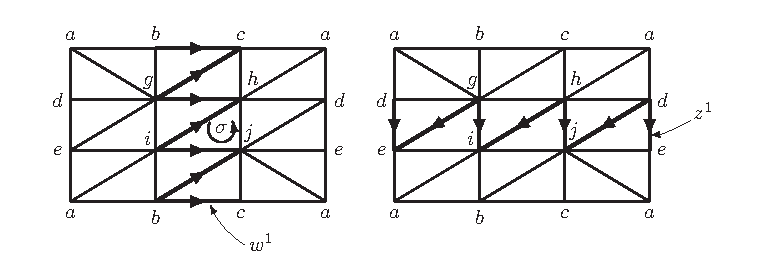
\includegraphics[width=.96\textwidth]{figures/8-8-1.pdf}
\caption*{图 8.8.1}
\end{figure}

\sourcepage{483--484}
定理的证明也说明为何应当如此。从 $w^1$ 出发，几何对偶映射 $\psi$ 将它映到图 8.8.2 中的闭链 $c_1$。该链承载于 $w^1$ 支承单形的对偶块中；要确认符号为 $c_1$ 而不是 $-c_1$，需要仔细检验。它与矩形侧边的胞腔 $B$ 所代表闭链同调。再通过代数对偶，$B$ 对应于在 $B$ 上取 $1$、在另一方向闭链 $A$ 上取 $0$ 的上闭链，$z^1$ 正是这样的上闭链。因此组合对偶把 $w^1$ 对应到 $z^1$，与 $\{z^1\smile w^1\}=\Lambda$ 以及两者的平方均为零相符。

\begin{figure}[htbp]\centering
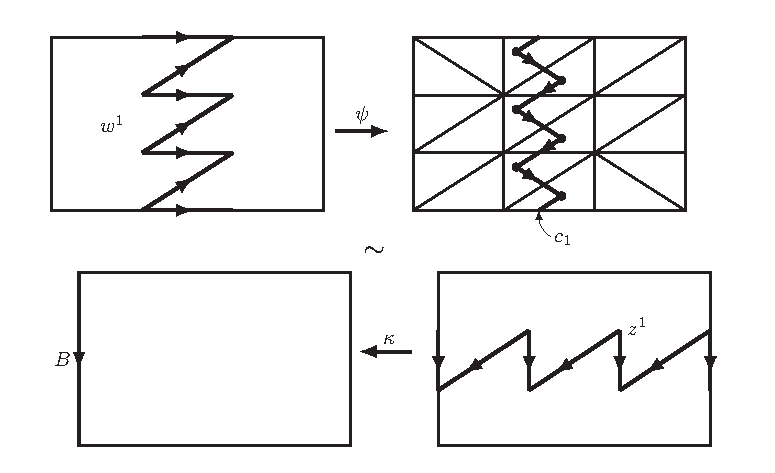
\includegraphics[width=.96\textwidth]{figures/8-8-2.pdf}
\caption*{图 8.8.2}
\end{figure}

现在研究实射影空间 $P^n$。它可三角剖分（引理 4.14.11），所以可用对偶定理。其胞腔链群在 $0\le k\le n$ 每维为 $\Z$，边缘为零或乘以 $2$，因此 $H^k(P^n;\Z/2)$ 在这些维数均为一维。还需计算杯积。以下用 $u^r$ 表示 $r$ 个 $u$ 的重复杯积。

\entry{定理}{8.8.5}若 $u$ 是 $H^1(P^n;\Z/2)$ 的非零元，则 $u^k$ 是 $H^k(P^n;\Z/2)$ 的非零元，$2\le k\le n$。因此
\[H^*(P^n;\Z/2)\cong(\Z/2)[u]/(u^{n+1}),\qquad\deg u=1.\]
即这是一个以一维元生成、在 $n+1$ 次截断的多项式代数。

\textbf{证明：}从 $n=2$ 开始归纳。此时 $H^1$ 一维，由定理 8.8.3，唯一非零元 $u$ 必满足 $u^2\ne0$。假定对 $n-1$ 成立。包含 $P^{n-1}\to P^n$ 在低于 $n$ 维诱导 $\Z/2$ 系数上同调同构，且保持杯积，所以 $u,u^2,\ldots,u^{n-1}$ 均非零。由定理 8.8.3，一维群 $H^1$ 和 $H^{n-1}$ 的生成元之积必须生成 $H^n$；它们唯一的非零元分别是 $u,u^{n-1}$，故 $u^n\ne0$。\hfill$\square$

\entry{推论}{8.8.6}$H^*(P^\infty;\Z/2)$ 是以一个一维元生成的多项式代数。

\textbf{证明：}包含 $P^n\to P^\infty$ 在不高于 $n$ 维诱导上同调同构，且保持杯积。\hfill$\square$

接着证明几个经典拓扑定理。

\entry{定义}{8.8.7}若映射满足 $f(-x)=-f(x)$，则称其\emph{保持对径点}。

\entry{定理}{8.8.8}若 $f:S^n\to S^m$ 连续且保持对径点，则 $n\le m$。

\sourcepage{485}
\textbf{证明：}记 $a_n=(1,0,\ldots,0)\in S^n$ 为基点，$F=\Z/2$。

第一步：设 $\pi_n:S^n\to P^n$ 是通常商映射。若 $\alpha$ 为从 $a_n$ 到 $-a_n$ 的任意道路，则 $\pi_n\alpha$ 代表 $H_1(P^n;F)$ 的非零元。

\begin{figure}[htbp]\centering
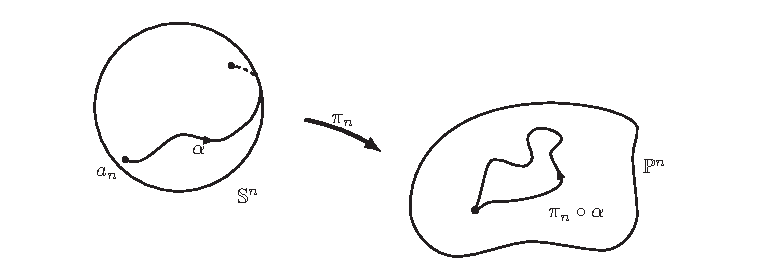
\includegraphics[width=.96\textwidth]{figures/8-8-3.pdf}
\caption*{图 8.8.3}
\end{figure}

先取标准道路 $\beta(t)=(\cos\pi t,\sin\pi t,0,\ldots,0)$。它把 $(I,\Bd I)$ 同胚到上半圆及其端点。$\pi_1$ 将端点粘合，映到 $(P^1,P^0)$。由 CW 复形的基本结果，相对生成元的像为一维胞腔的基本闭链，故 $\pi_n\beta$ 生成 $H_1(P^n;F)$。

一般地，$\alpha-\beta$ 是 $S^n$ 中的奇异闭链。若 $n>1$，$H_1(S^n)=0$，所以它是某二维链 $d$ 的边界。于是 $\pi_n\alpha-\pi_n\beta=\partial(\pi_{n\#}d)$，二者同调。若 $n=1$，商映射的度为 $2$，因此该差的像代表整数生成元的偶数倍，模 $2$ 后仍为零。第一步得证。

\sourcepage{486}
第二步：将 $f$ 与目标球面的旋转 $\rho$ 复合，使 $g=\rho f$ 把 $a_n$ 映到 $a_m$。它仍保持对径点，因而诱导 $h:P^n\to P^m$，满足 $h\pi_n=\pi_mg$。若 $\alpha$ 从 $a_n$ 通向 $-a_n$，则 $g\alpha$ 从 $a_m$ 通向 $-a_m$。由第一步，$h_*$ 把一维同调的非零元映到非零元。

第三步：由 Kronecker 同构的自然性，$h^*:H^1(P^m;F)\to H^1(P^n;F)$ 也非零。若 $u$ 为源的非零元，则 $h^*u$ 为目标的非零元。保持杯积给出
\[h^*(u^n)=(h^*u)^n\ne0.\]
故 $u^n\ne0$，从而 $m\ge n$。\hfill$\square$

\entry{定理}{8.8.9（Borsuk--Ulam 定理）}若 $h:S^n\to\R^n$ 连续，则存在 $x$ 使 $h(x)=h(-x)$。

\textbf{证明：}否则
\[f(x)=\frac{h(x)-h(-x)}{\|h(x)-h(-x)\|}\]
给出连续且保持对径点的 $S^n\to S^{n-1}$ 映射，与上一定理矛盾。\hfill$\square$

\entry{定理}{8.8.10（初等形式的火腿三明治定理）}平面中任意两个有界可测集合 $A_1,A_2$，可被同一直线按面积同时二等分。

\entry{注}{8.8.11}这个结论并不初等。即使两个集合都是三角区域，也可以试着寻找这样的直线。

\sourcepage{487}
\textbf{证明：}把平面视为 $\R^3$ 中的 $\R^2\times\{1\}$。对单位向量 $u\in S^2$，令 $P(u)$ 为过原点且垂直于 $u$ 的平面；$f_i(u)$ 为 $A_i$ 位于 $P(u)$ 的 $u$ 一侧的部分的测度。于是
\[f_i(u)+f_i(-u)=\operatorname{measure}(A_i).\]
映射 $u\mapsto(f_1(u),f_2(u))$ 连续。由 Borsuk--Ulam 定理，存在 $a$ 使 $f_i(a)=f_i(-a)$，从而均等于 $A_i$ 测度的一半。$P(a)$ 与原平面的交线就是所需直线。\hfill$\square$

\begin{figure}[htbp]\centering
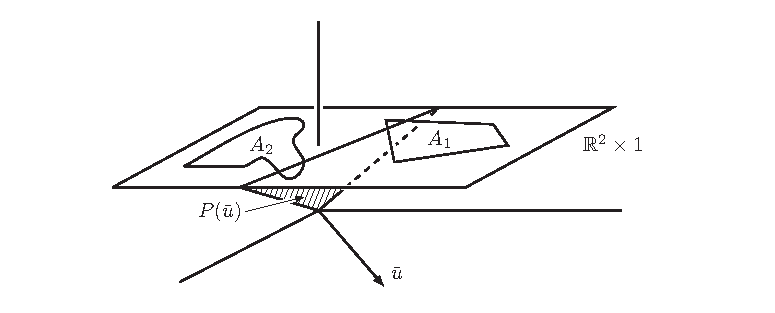
\includegraphics[width=.96\textwidth]{figures/8-8-4.pdf}
\caption*{图 8.8.4}
\end{figure}

证明可直接推广：$\R^n$ 中任意 $n$ 个有界可测集合，都可被同一 $(n-1)$ 维超平面同时二等分。名称来自三维情形：把三明治想成两片面包夹一片火腿，一刀即可同时把三片各自平分。

\sourcepage{488--489}
\subsection*{习题}
\begin{enumerate}
\item 设 $T$ 如例 8.8.4，$g:\operatorname{sd}T\to T$ 是恒等映射的单纯逼近。令 $\operatorname{sd}\gamma$ 为所有逆时针定向二维单形之和，验证 $g^\#w^1\frown\operatorname{sd}\gamma$ 为图 8.8.2 的 $c_1$。
\item \begin{enumerate}[label=(\alph*)]
\item 若 $\varphi:R\to R'$ 是有单位元交换环之间的同态，证明诱导的 $H^*(X;R)\to H^*(X;R')$ 为环同态。
\item 用系数同态 $\Z\to\Z/2$ 计算 $P^{2k},P^{2k+1},P^\infty$ 的整数上同调环。
\end{enumerate}
\item 证明任意时刻，地球表面都有一对对径点，其温度与气压分别相同。
\item 计算：(a) $S^3\times P^5$ 的 $\Z$ 及 $\Z/2$ 系数上同调环；(b) $P^2\times P^3$ 的 $\Z/2$ 系数上同调环。
\item 假设 $\mathbb{CP}^n$ 可三角剖分（事实上确实可以）。
\begin{enumerate}[label=(\alph*)]
\item 计算 $H^*(\mathbb{CP}^n)$ 和 $H^*(\mathbb{CP}^\infty)$。
\item 对 $f:\mathbb{CP}^n\to\mathbb{CP}^n$，证明其度为某整数 $a$ 的 $n$ 次方。
\item 证明 $\mathbb{CP}^{2n}$ 的每个自映射都有不动点。
\item 证明不存在度为 $-1$ 的 $\mathbb{CP}^{2n}$ 自映射。
\item 若 $\mathbb{CP}^{2n+1}$ 的自映射无不动点，其度是多少？
\end{enumerate}
\item 〔*〕从两个 $\mathbb{CP}^2$ 各删去一个小开四维球，再沿边界三维球面粘合得到流形 $M$。讨论其上同调环，并与 $S^2\times S^2$ 比较。
\item 设 $X$ 为连通、可三角剖分的同调七维流形，满足
\[H^7(X)\cong\Z,\quad H^6(X)\cong\Z,\quad H^5(X)\cong\Z/2,\quad
H^4(X)\cong\Z\oplus\Z/3.\]
尽可能确定其他上同调群及环结构。
\item 设 $X$ 是紧致可定向、可三角剖分的同调 $(4n+2)$ 维流形。证明不可能有 $H^{2n+1}(X)\cong\Z$。
\item 令 $X_0=S^2$，$X_n$ 为 $n$ 个环面的连通和，$Y_n$ 为 $n$ 个射影平面的连通和。考察 $f_*$ 在 $\Z/2$ 系数二维同调上非零这一条件。
\begin{enumerate}[label=(\alph*)]
\item 证明不存在满足条件的 $Y_{2n}\to X_n$。〔提示：自由群之间的同态，若源秩大于目标秩，则核有正秩且为直和分量。选择 $H^1(X_n)$ 的基使 $f^*(\beta_1)=0$，再转为模 $2$ 系数，应用定理 8.8.3 的证明。〕
\item 证明存在满足条件的 $Y_{2n+1}\to X_n$。〔提示：先证 $Y_3\approx T\mathbin{\#}P^2$。〕
\item 证明存在满足条件的 $Y_m\to X_n$，当且仅当 $m\ge2n+1$。
\end{enumerate}
\item 举出不保持对径点的连续映射 $S^2\to S^2$。每个维数都有这样的例子吗？
\item 表述四维空间中的火腿三明治定理，并尝试证明。
\end{enumerate}
